%%\documentclass[aps,twocolumn]{article}%
%%\usepackage{graphicx}
%%\begin{document}
\label{sec:PE}
\section {PhotoElectronics}

%({\it eugenio.scapparone@bo.infn.it})  \\

%%\subsection {Introduction}
Following the successful construction of the first Photo-Detector Module (PDM) on March 2018, the DarkSide Photo-Electronic group proceeded to the construction of the first Motherboard, made by 25 PDMs,
each equipped with 24 rectangular SiPMs (11.7 x 7.9 mm).
The FBK company~\cite{FBK:2018a}  delivered two SiPM runs: 
the first one with standard doping SiPMs (cell size 25 $\mu$m and quenching resistor 10 M$\Omega$(77 K)) and the second one with triple doping SiPMs (cell size 30 $\mu$m and quenching resistor 5 M$\Omega$(77 K)). Since the latter SiPM type is considered the best candidate for the DarkSide experiment, we decided to use for the first Motherboard construction 
the single doping SiPM, so that the triple doping type could be mounted later, taking advantage of the experience gained with the mounting of the first Motherboard.
\begin{figure} [t]
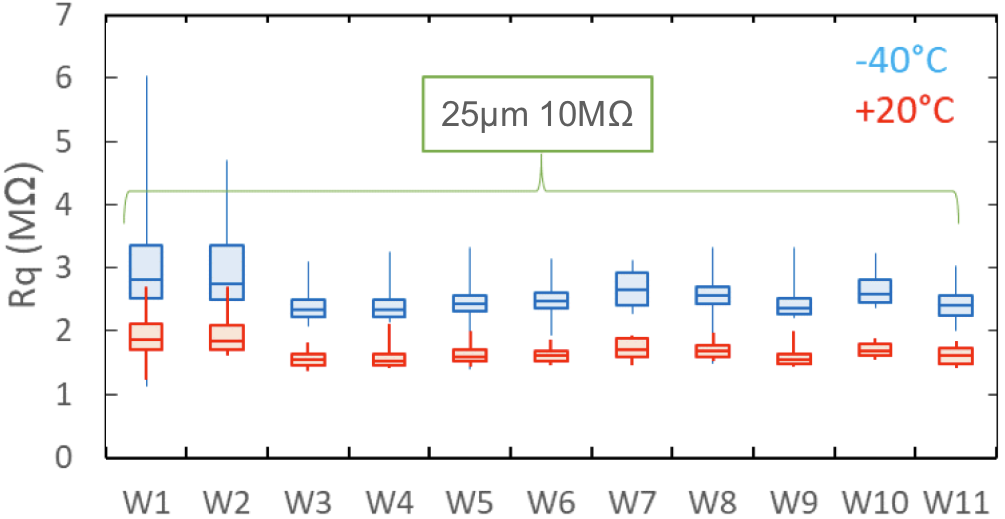
\includegraphics[width=0.99\columnwidth]{./Figures/Rq.png}
\caption{Average SiPM  quenching resistor  value vs wafer number measured at 20 and -40 degrees}
\label{fig:Rq} 
\end{figure} 
 This SiPM run was characterized by a reasonable yield at -40 degrees, about 50$\%$. A detailed inspection of the SiPM quenching resistor ($R_q$) showed a good uniformity for most of the wafers, while the first and the second wafers (W1,W2) had a 20$\%$ larger $R_q$ (see fig.\ref{fig:Rq}). The SiPM optimal working voltage is expected to change as a function of $R_q$: in the forthcoming  massive production by the LFoundry company~\cite{LFoundry:2018a}, where hundreds of 8" SiPM wafers are scheduled, this quenching resistor spread  is not an issue, since the SiPMs with similar $R_q$ can be paired; in this way each Motherboard, whose PDMs are fed at the same voltage, will be made of devices with similar $R_q$. 
Due the limited SiPMs available in the present production we had to use all of them to make the first Motherboard, fed with a common voltage. As a consequence the tiles made with SiPM belonging to wafers 1,2 were fed with a voltage lower than the optimal one, i.e. 5V. 
It is worth noting that a dedicated facility for the Motherboard production is not available yet: the use of equipment in outsourcing and an additional man power effort was therefore required.
The tile and the Front-End Board PCBs were made with an Arlon 55-NT~\cite{Arlon:2018a} substrate, following the experience gained during the first PDM construction. The electronic components were mounted in outsourcing, under the supervision of LNGS personnel. The tile PCBs were tested both at warm and at cryogenic temperatures to verify the correct circuit impedance. After the wafer dicing, the SiPMs were shipped from the FBK to the Princeton University, where
the first Motherboard tiles were bonded by personnel from LNGS, Princeton University and TIFPA. A cryogenic epoxy for the SiPM back-side and a wire-bonding connection for the front-side was used. The 27 tiles, each made of 24 SiPMs, were finally shipped to LNGS, using multipurpose acrylic boxes, designed by the Pisa group. This box allows a safe shipping of the tile, offering an appropriate protection of the SiPM wire bonding and, at the same, time allows the tile characterization in liquid nitrogen by permitting the insertion of the Front End Board without removing the tile from the box. The tiles underwent a comprehensive test at LNGS both at warm temperature and in LN, including the reverse I-V curve measurement, the power spectrum and the charge spectra. We found just one tile 
(n. 20) over 27 tiles with two SiPM branches (4 SiPMs) not working properly. Another tile (n.13) showed a noise level higher than the average. These two tiles were therefore excluded from the list of the tiles selected to populate the first Motherboard.
As an example Fig.\ref{fig:I-V} shows the tile I-V curves taken at 77 K, indicating a homogeneous behaviour.  
\begin{figure} [t]
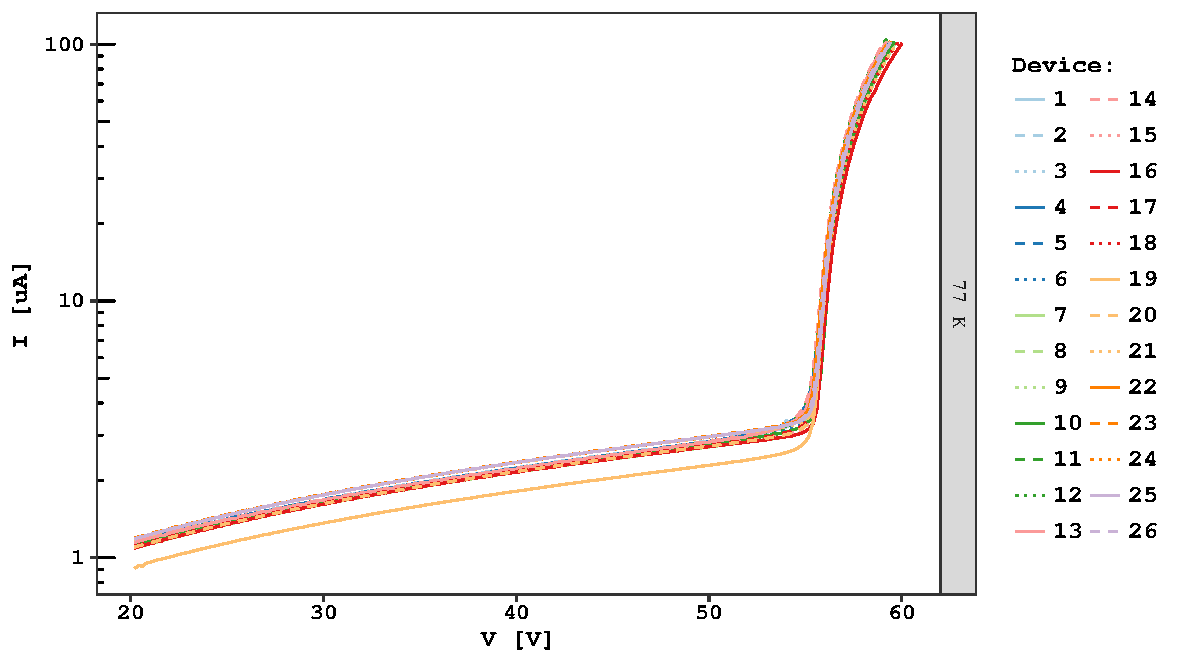
\includegraphics[width=0.99\columnwidth]{./Figures/IV_77K.pdf}
\caption{Reverse I-V curves of the tiles measured at 77K}
\label{fig:I-V} 
\end{figure} 
\begin{figure} [t]
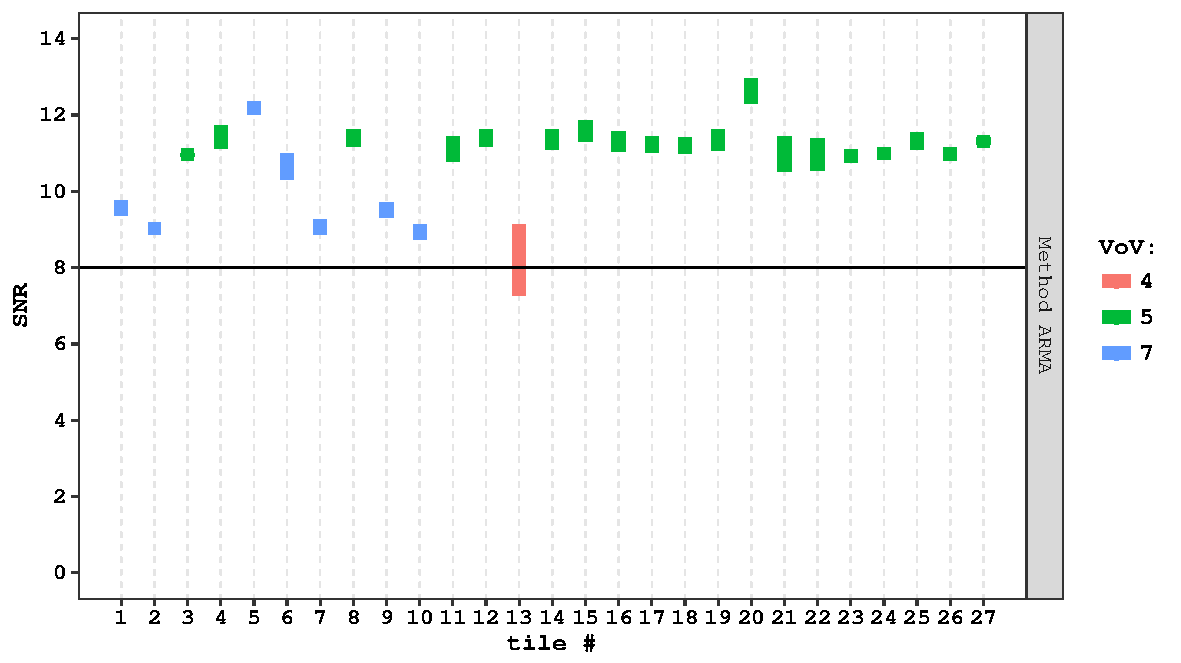
\includegraphics[width=0.99\columnwidth]{./Figures/SNR.pdf}
\caption{SNR of the 27 bonded SiPM tiles}
\label{fig:SNR} 
\end{figure} 
Fig.\ref{fig:SNR} shows the signal to noise ratio (SNR) for the 27 tiles at their optimal voltage: it is worth noting that all of them have a SNR larger than the minimum SNR = 8, required by the DarkSide-20k experiment specifications. For each tile the SNR was obtained relying on several different procedures and analysis method: the bar length in the figure represents the spread of each measurement, depending on the used method. 
The signal-to-noise ratio (SNR) is defined as the ratio between the gain and the baseline noise. The gain is measured by fitting the center values of the amplitude multiple peaks and evaluating the slope of a linear fit. The baseline noise is extracted from the average standard deviation of the waveform in a pre-pulse window, 500 ns long, using 500 samples. For most tiles, the distribution of the standard deviation is not symmetric around the peak: the most important contribution to the noise baseline is the presence of one of more photoelectrons not stimulated by the laser pulse. These can be originated by a SiPM having an excess of dark-rate or more probably by an excess of after-pulse. 
Since the distribution is not symmetric, the estimate of the baseline noise is intrinsically biased and two options are possible, corresponding to the mean value or the most probable value (mode). Consequently the SNR is defined in a confidence interval between $SNR_{min}$ = gain/$noise_{mean}$
and $SNR_{max}$  = gain/$noise_{mode}$.
\begin{figure} [t]
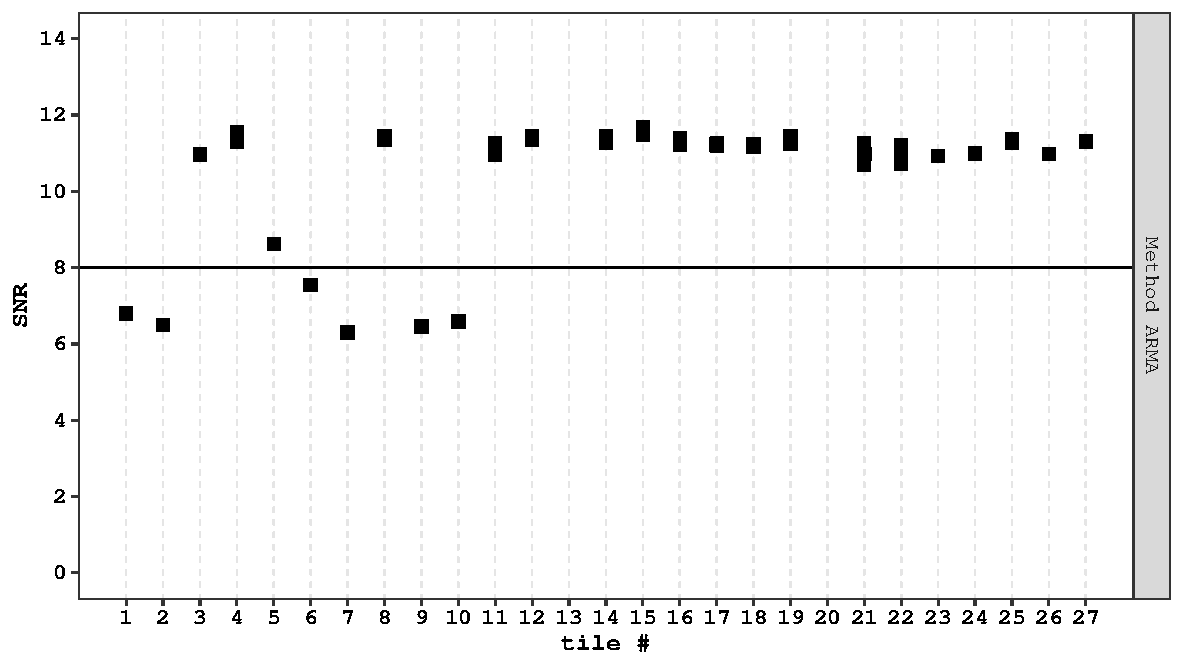
\includegraphics[width=0.99\columnwidth]{./Figures/SNR2.pdf}
\caption{SNR of the 25 SiPM tiles selected to populate the first motherboard operate at an over-voltage of 5V.}
\label{fig:SNR2} 
\end{figure} 

Fig.\ref{fig:SNR2} shows the SNR obtained with the common over-voltage of 5V. Although few tiles, as expected, manifest a SNR slightly below 8, the overall Motherboard SNR is quite good.
Before assembling the first Motherboard, a full mock-up made of an aluminium Motherboard structure, a FR4 Motherboard strip PCB, 25 dummy tiles and FEBs, and the PDM acrylic mechanics, was mounted at Bologna. Each PCB had the same dimensions of the final one, while the HV/LV and signal layers were not included in the stack-up. The mounting required just few hours and the overall procedure was validated: the mechanics of the different components nicely merged, suggesting just few minor mechanical improvements. 
After these tests the tiles were finally shipped to Pisa; the PDM pillars and the copper Motherboard structure were milled at Bologna, using a pure copper (99.997 $\%$) sold by Luvata company~\cite{Luvata:2018a} . The first Motherboard was equipped with a PCB strip connecting the PDMs, made of a thin stack-up (0.5 mm) based on a Pyralux~\cite{Pyralux:2018a} substrate and shipped to Pisa to start the mounting of the 25 PDMs on the Motherboard. 
The PDMs were assembled in the Pisa clean room, following the prescriptions used for the the first PDM, assembled in March 2018. 
The mounting of the 25 PDMs on the Motherboard started the third week of September and was finalized in few days.
Fig.\ref{fig:MB-photo} shows the Motherboard fully equipped with the 25 PDMs.
\begin{figure} [t]
\includegraphics[angle=270,width=0.99\columnwidth]{./Figures/MB-foto.jpg}
\caption{The first assembled  Motherboard}
\label{fig:MB-photo} 
\end{figure} 
%%

In summary the construction of the first Motherboard required the production, the test, the selection and the bonding of more than 600 SiPMs. Although a cryogenic probe and an automatic bonder were not available yet, the DarkSide Collaboration was able to increase the number of successfully built PDMs from 1 to 25, just in 6 months. The bonding yield was quite large, exceeding 95$\%$ (just 1 tile over 27 showed problems with SiPM bonding), while the satisfactory PDM SNR demonstrated the validity of the full Motherboard construction process.


%\end{document}
